\documentclass{beamer}

\usepackage[utf8]{inputenc}
%\usepackage{default}

\usetheme{Berlin}

\title{Imagerie Médicale}
\subtitle{Ingénierie d'une application}
\author{Jérôme Velut}
\date{04/12/2013}

\begin{document}

\frame{\titlepage}

\section*{Sommaire}
\begin{frame}{Sommaire}
  \tableofcontents[hideallsubsections]
\end{frame}

\section{Imagerie médicale}
\subsection{Bref historique}
\begin{frame}{Médecine nucléaire}
\begin{columns}[T]
 \begin{column}{0.5\textwidth}
 \centering
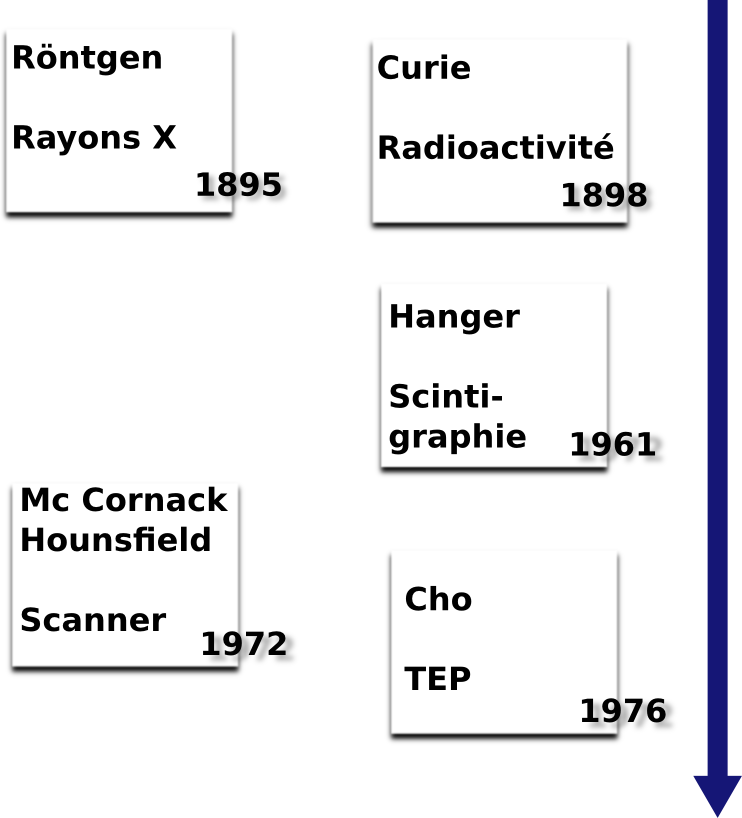
\includegraphics[height=0.7\textheight]{images/historique_radio.png}
 \end{column}
 \begin{column}{0.5\textwidth}
\begin{itemize}
 \item Médecine nucléaire: imageries, traitements par rayonnement ionisant
 \item Applications industrielles également
 \item Effets sur la santé
\end{itemize}
 \end{column}
\end{columns}
\end{frame}
\begin{frame}{Médecine nucléaire}
\begin{columns}[T]
 \begin{column}{0.5\textwidth}
 \centering
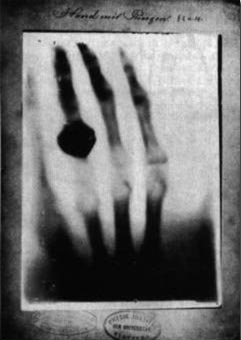
\includegraphics[height=0.7\textheight]{images/main_roentgen.jpg}\\
Première radiographie
 \end{column}
 \begin{column}{0.5\textwidth}
 \centering
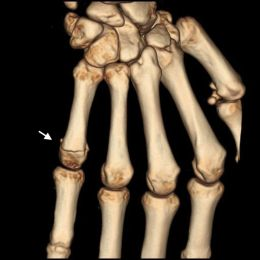
\includegraphics[height=0.5\textheight]{images/main_TDM.jpg}\\
Scanner haute résolution (fracture)
 \end{column}
\end{columns}
\end{frame}
\begin{frame}{Résonance magnétique}
\begin{columns}[T]
 \begin{column}{0.5\textwidth}
 \centering
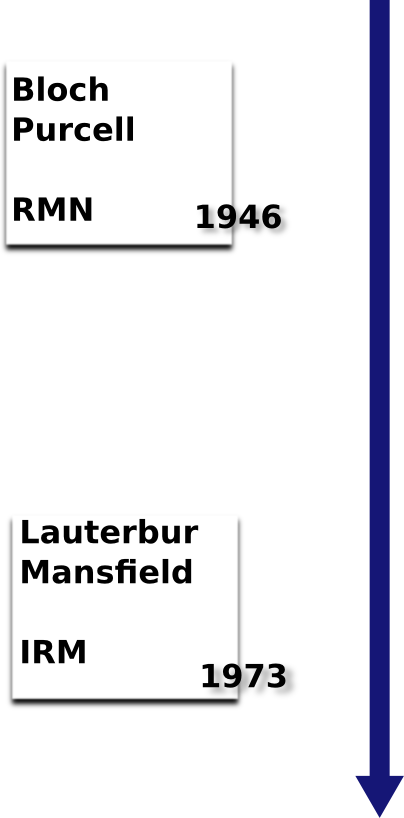
\includegraphics[height=0.7\textheight]{images/historique_rmn.png}
 \end{column}
 \begin{column}{0.5\textwidth}
\begin{itemize}
 \item Emission d'une onde radiofréquence par les noyaux placés dans un champ magnétique
 \item Spectroscopie RMN : observation de différents isotopes
 \item IRM: observation de l'hydrogène
\end{itemize}
 \end{column}
\end{columns} 
\end{frame}
\begin{frame}{Résonance magnétique}
\begin{columns}[T]
 \begin{column}{0.5\textwidth}
 \centering
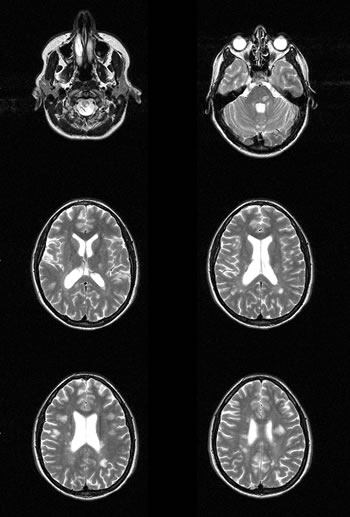
\includegraphics[height=0.6\textheight]{images/irm_t2.jpg}\\
IRM pondération T1
 \end{column}
 \begin{column}{0.5\textwidth}
 \centering
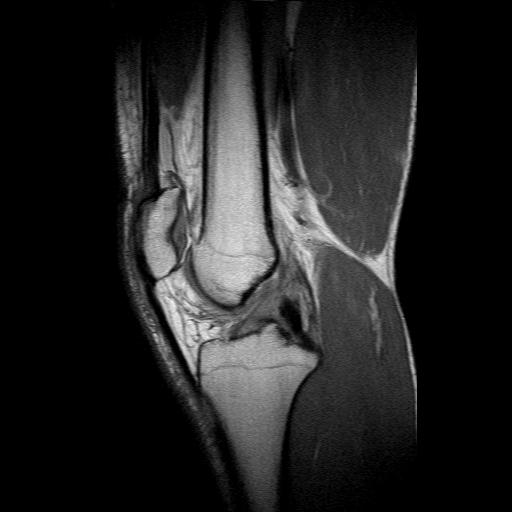
\includegraphics[height=0.6\textheight]{images/IRM_genou_sag_2.png}\\
IRM pondération T2
 \end{column}
\end{columns} 
\end{frame}

\begin{frame}{Ultrasons}
 \begin{columns}[T]
 \begin{column}{0.5\textwidth}
 \centering
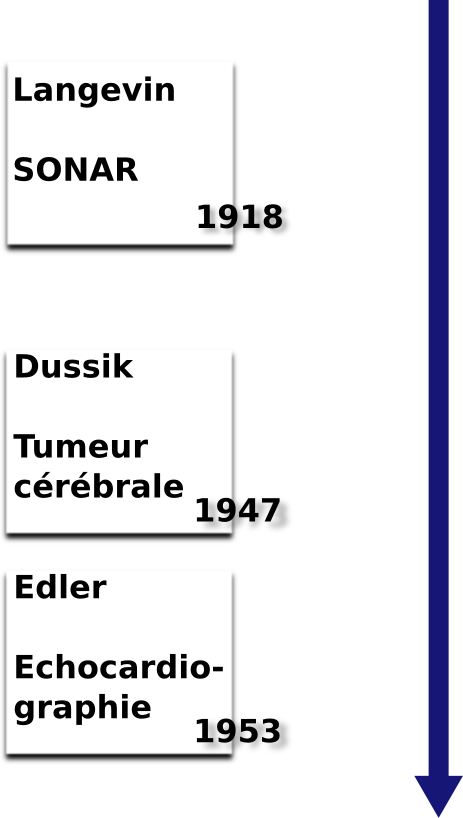
\includegraphics[height=0.7\textheight]{images/historique_us.png}
 \end{column}
 \begin{column}{0.5\textwidth}
\begin{itemize}
 \item Mesure la reflexion des ondes ultrasonores
 \item Effet Doppler : mesure de vitesse
 \item Portable, non invasif, innocuité++
\end{itemize}
 \end{column}
\end{columns} 
\end{frame}
\begin{frame}{Ultrasons}
 \begin{columns}[T]
 \begin{column}{0.32\textwidth}
 \centering
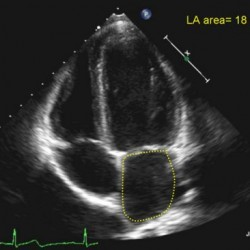
\includegraphics[width=0.9\textwidth]{images/echocardio.jpg}\\
Echographie cardiaque
 \end{column}
 \begin{column}{0.32\textwidth}
 \centering
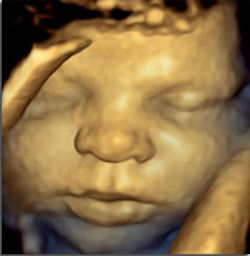
\includegraphics[width=0.9\textwidth]{images/echo3d.jpg}\\
Obstétrique
 \end{column}
 \begin{column}{0.32\textwidth}
 \centering
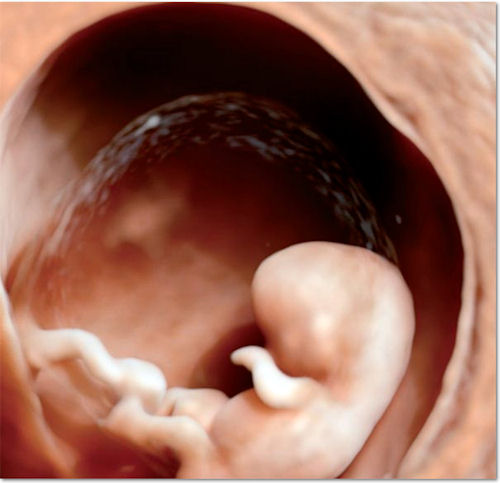
\includegraphics[width=0.9\textwidth]{images/echo3dhd.jpg}\\
Avec un bon traitement d'image...
 \end{column}\end{columns} 
\end{frame}
\subsection{Méthodes de diagnostic}
\begin{frame}{Diagnostic}
\begin{itemize}
 \item Diagnostic = identifier les causes des symptômes (étiologie) en vue d'adapter le traitement
 \item US, IRM, TDM: imagerie anatomique (ou structurelle)
 \item USf, IRMf, TEP: imagerie fonctionnelle
 \item Rôle de l'imagerie: exploration - décision
\end{itemize}
\end{frame}

\begin{frame}{Diagnostic}
  \begin{columns}[t]
 \begin{column}{0.5\textwidth}
 \begin{block}{Exploration}
  \begin{itemize}
   \item Recherche de pathologies
   \item $\rightarrow$ Segmentations
   \item $\rightarrow$ Interactions
  \end{itemize}
 \end{block}
 \end{column}
 \begin{column}{0.5\textwidth}
 \begin{block}{Décision}
  \begin{itemize}
   \item Adaptation du traitement
   \item $\rightarrow$ Quantifications
  \end{itemize}
 \end{block}
\end{column}
\end{columns}
\end{frame}

\subsection{Thérapie guidée par l'image}
\begin{frame}{Principes}
\centering
  \begin{columns}[t]
 \begin{column}{0.5\textwidth}
\begin{block}{Améliorer la précision}
\begin{itemize}
  \item localisation
  \item dose
 \end{itemize}
\end{block}
 \end{column}
 \begin{column}{0.5\textwidth}
\begin{block}{Diminuer les traumatismes}
\begin{itemize}
  \item Interventions non (mini) invasives
  \item gestes chirurgicaux plus rapides
  \end{itemize}
\end{block}
\end{column}
\end{columns}
  \item (\small$\rightarrow$ robotique médicale)
\end{frame}
\begin{frame}{Planification}
 \centering
  \begin{columns}[t]
 \begin{column}{0.5\textwidth}
\begin{block}{Planification}
\begin{itemize}
 \item Prévoir l'intervention (par ex. dépôt de dose)
 \item Imagerie anatomique et/ou fonctionnelle : localisation
 \item Modification topologique lors de l'intervention
\end{itemize}\end{block}
 \end{column}
 \begin{column}{0.5\textwidth}
\begin{block}{Guidage par l'image}
\begin{itemize}
  \item Modification de la planification en cours de traitement
  \item $\rightarrow$ Moins de traitement
  \item $\rightarrow$ Plus efficace
  \end{itemize}
\end{block}
\end{column}
\end{columns}
\end{frame}

\begin{frame}{Couplages}
 
\end{frame}

\subsection{Thérapie par ultrasons focalisés de haute intensité}
\begin{frame}{Indications}
 
\end{frame}

\begin{frame}{Technologie}
 
\end{frame}

\begin{frame}{Apport de l'IRM}
 
\end{frame}


\section{Recalage d'images}
\subsection{Objectifs}
\begin{frame}{Mise en correspondance}
 
\end{frame}

\subsection{Méthode}
\begin{frame}{Vue globale}
 
\end{frame}
\begin{frame}{Métrique}
 
\end{frame}

\subsection{Recalage multimodal}
\begin{frame}{Information mutuelle}
 
\end{frame}
\begin{frame}{Limitation}
 
\end{frame}

\subsection{Recalage basé modèle}
\begin{frame}{Entrées}
 
\end{frame}
\begin{frame}{Similarité}
 
\end{frame}

\section{Autres applications}
\subsection{Stabilisation de vidéos}
\begin{frame}{Stabilisation}
 
\end{frame}

\subsection{Segmentation basée sur des atlas}
\begin{frame}{Segmentation}
 
\end{frame}
\subsection{Interpolation}
\begin{frame}{Interpolation}
 
\end{frame}


\end{document}
